\documentclass[12pt,a4paper]{report}

% --- Языковые настройки и шрифты (XeLaTeX) ---
\usepackage{fontspec}
\setmainfont{Times New Roman}
\newfontfamily\cyrillicfont{Times New Roman}
\setmonofont{Courier New}
\newfontfamily\cyrillicfonttt{Courier New}

\usepackage{polyglossia}
\setdefaultlanguage{russian}
\setotherlanguage{english}

% --- Геометрия страницы ---
\usepackage{geometry}
\geometry{
    top=20mm,
    bottom=20mm,
    left=25mm,
    right=15mm,
    headheight=15pt,
    footskip=10mm
}

% --- Пакеты оформления и графики ---
\usepackage{xcolor}
\definecolor{primaryblue}{RGB}{24, 75, 145}
\definecolor{darkslate}{RGB}{15, 23, 42}
\definecolor{accentgreen}{RGB}{16, 149, 100}
\definecolor{accentred}{RGB}{200, 35, 45}
\definecolor{cardbg}{RGB}{248, 250, 252}
\definecolor{cardborder}{RGB}{203, 213, 225}

\usepackage{graphicx}
\graphicspath{{images/}}

\usepackage{tabularx}
\usepackage{booktabs}
\usepackage{array}
\usepackage{float}
\usepackage{caption}
\captionsetup{
    font=small,
    labelfont={bf,color=primaryblue},
    justification=centering,
    skip=8pt
}

% --- Красивые врезки (tcolorbox) ---
\usepackage{tcolorbox}
\tcbuselibrary{skins,breakable}

\newtcolorbox{infoNote}[1][]{
    enhanced,
    colback=primaryblue!5!white,
    colframe=primaryblue,
    fonttitle=\bfseries\color{white},
    title=Методическое указание,
    arc=4mm,
    boxrule=1pt,
    left=12pt,
    right=12pt,
    top=8pt,
    bottom=8pt,
    before skip=12pt,
    after skip=12pt,
    #1
}

\newtcolorbox{warnBox}[1][]{
    enhanced,
    colback=accentred!5!white,
    colframe=accentred,
    fonttitle=\bfseries\color{white},
    title=Внимание / Ограничение безопасности,
    arc=4mm,
    boxrule=1pt,
    left=12pt,
    right=12pt,
    top=8pt,
    bottom=8pt,
    before skip=12pt,
    after skip=12pt,
    #1
}

\newtcolorbox{tipBox}[1][]{
    enhanced,
    colback=accentgreen!5!white,
    colframe=accentgreen,
    fonttitle=\bfseries\color{white},
    title=Практическая рекомендация,
    arc=4mm,
    boxrule=1pt,
    left=12pt,
    right=12pt,
    top=8pt,
    bottom=8pt,
    before skip=12pt,
    after skip=12pt,
    #1
}

% --- Колонтитулы ---
\usepackage{fancyhdr}
\pagestyle{fancy}
\fancyhf{}
\fancyhead[L]{\small\color{darkslate}\textit{Комплекс имитационного моделирования «Смальта» (Релиз 2.2.0)}}
\fancyhead[R]{\small\color{primaryblue}\textbf{Руководство по эксплуатации}}
\fancyfoot[C]{\thepage}
\renewcommand{\headrulewidth}{0.5pt}
\renewcommand{\footrulewidth}{0.4pt}

% --- Гиперссылки ---
\usepackage{hyperref}
\hypersetup{
    colorlinks=true,
    linkcolor=primaryblue,
    filecolor=primaryblue,
    urlcolor=primaryblue,
    citecolor=primaryblue,
    pdftitle={Методическое руководство по эксплуатации симулятора РЭБ «Смальта» и сетевой подсистемы «Клиент-Преподаватель»},
    pdfauthor={Военный Учебный Центр / Кафедра РЭБ},
    pdfsubject={Руководство по эксплуатации и проведению экзаменов},
    pdfkeywords={Смальта, РЭБ, Симулятор, PyGame, Клиент-Преподаватель, Мониторинг, Экзамен}
}

% Устранение переносов в заголовках
\usepackage{titlesec}
\titleformat{\chapter}[display]
  {\normalfont\huge\bfseries\color{primaryblue}}{\chaptertitlename\ \thechapter}{16pt}{\Huge}
\titleformat{\section}
  {\normalfont\Large\bfseries\color{primaryblue}}{\thesection}{1em}{}
\titleformat{\subsection}
  {\normalfont\large\bfseries\color{darkslate}}{\thesubsection}{1em}{}

\begin{document}

% =========================================================================
% ТИТУЛЬНЫЙ ЛИСТ
% =========================================================================
\begin{titlepage}
    \centering
    {\large\bfseries МИНИСТЕРСТВО НАУКИ И ВЫСШЕГО ОБРАЗОВАНИЯ РОССИЙСКОЙ ФЕДЕРАЦИИ}\\[4mm]
    {\normalsize ВОЕННЫЙ УЧЕБНЫЙ ЦЕНТР}\\[2mm]
    {\normalsize КАФЕДРА РАДИОЭЛЕКТРОННОЙ БОРЬБЫ И ТЕХНИЧЕСКОЙ ЗАЩИТЫ ИНФОРМАЦИИ}\\[25mm]

    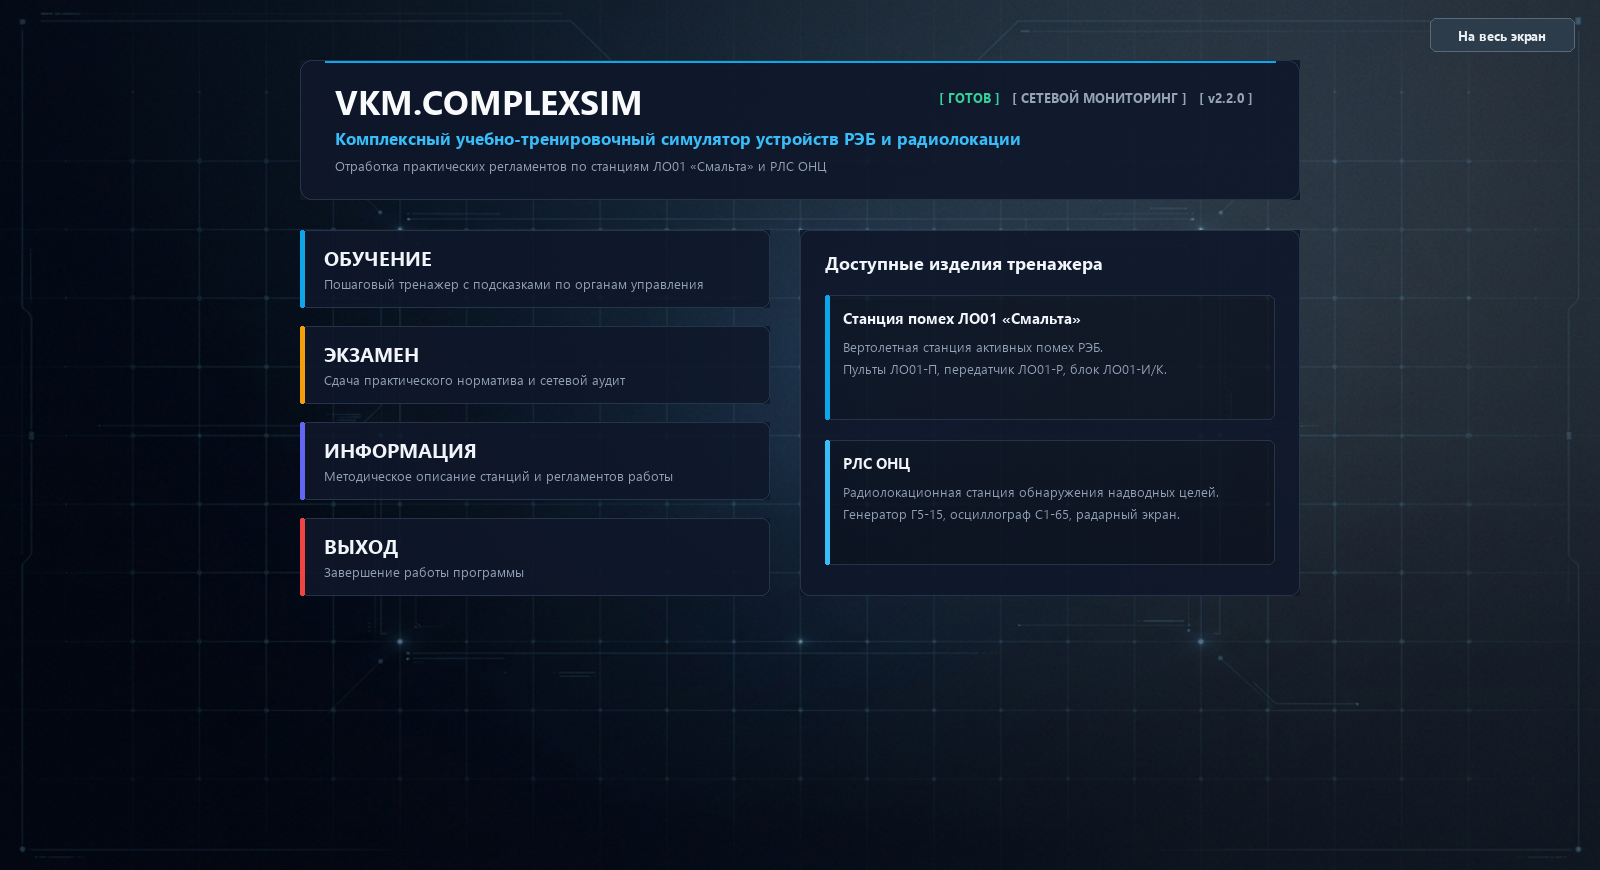
\includegraphics[width=0.28\textwidth]{01_main_menu.png}\\[8mm]

    {\Huge\bfseries\color{primaryblue} ПРОГРАММНЫЙ КОМПЛЕКС\\[3mm]
    ИМИТАЦИОННОГО МОДЕЛИРОВАНИЯ И СЕТЕВОГО КОНТРОЛЯ ЗНАНИЙ}\\[6mm]

    {\Large\bfseries СИМУЛЯТОР СТАНЦИИ ПОМЕХ РЭБ «СМАЛЬТА»}\\[4mm]
    {\large\bfseries (Версия 2.2.0)}\\[12mm]

    \begin{tcolorbox}[enhanced,colback=cardbg,colframe=primaryblue,arc=3mm,width=0.92\textwidth,center]
        \centering
        \textbf{\large МЕТОДИЧЕСКОЕ РУКОВОДСТВО}\\[2mm]
        \normalsize по развёртыванию, эксплуатации и проведению автоматизированных экзаменов в распределённой архитектуре «Клиент-Преподаватель»
    \end{tcolorbox}

    \vfill

    \begin{flushright}
        \parbox{0.45\textwidth}{
            \small
            \textbf{Разработчик:}\\
            Группа моделирования ВУЦ\\
            \textbf{Ревизия ПО:} v2.2.0 (Release)\\
            \textbf{Среда исполнения:} Windows x64
        }
    \end{flushright}

    \vspace{8mm}
    {\small 2026 год}
\end{titlepage}

% =========================================================================
% ОГЛАВЛЕНИЕ
% =========================================================================
\tableofcontents
\newpage

% =========================================================================
% ГЛАВА 1: ВВЕДЕНИЕ
% =========================================================================
\chapter{Введение и назначение программного комплекса}

\section{Общие сведения}
Программный комплекс имитационного моделирования \textbf{SmaltaSim} представляет собой интерактивный аппаратно-ориентированный тренажёр, предназначенный для качественной теоретической и практической подготовки курсантов, слушателей и операторов специальной техники радиоэлектронной борьбы (РЭБ). 

Основная дидактическая цель комплекса --- формирование твёрдых двигательно-когнитивных навыков работы с панелями реальной аппаратуры, точное усвоение алгоритмов предпускового контроля, настройки частотных каналов, ввода станции в боевой режим работы и оперативного устранения неисправностей.

\section{Имитируемая материальная часть}
В составе программного комплекса реализована трёхмерно-плоскостная фотореалистичная модель стойки аппаратуры изделия \textbf{Л001 («Смальта»)}, включающая:
\begin{itemize}
    \item \textbf{Блок управления и индикации Л001-П}: основные коммутационные элементы питания, тумблеры подачи накала и высокого напряжения, кнопки контроля исправности каналов, селекторы имитатора излучения и стрелочные индикаторы токов каналов;
    \item \textbf{Приёмо-передающий блок Л003}: элементы высокочастотного тракта, тумблеры согласования антенных решёток, калибровочные узлы;
    \item \textbf{Вспомогательные пульты}: автоматы защиты сети (АЗС), органы управления охлаждением, вентиляцией и подсветкой рабочего стола.
\end{itemize}

\begin{figure}[H]
    \centering
    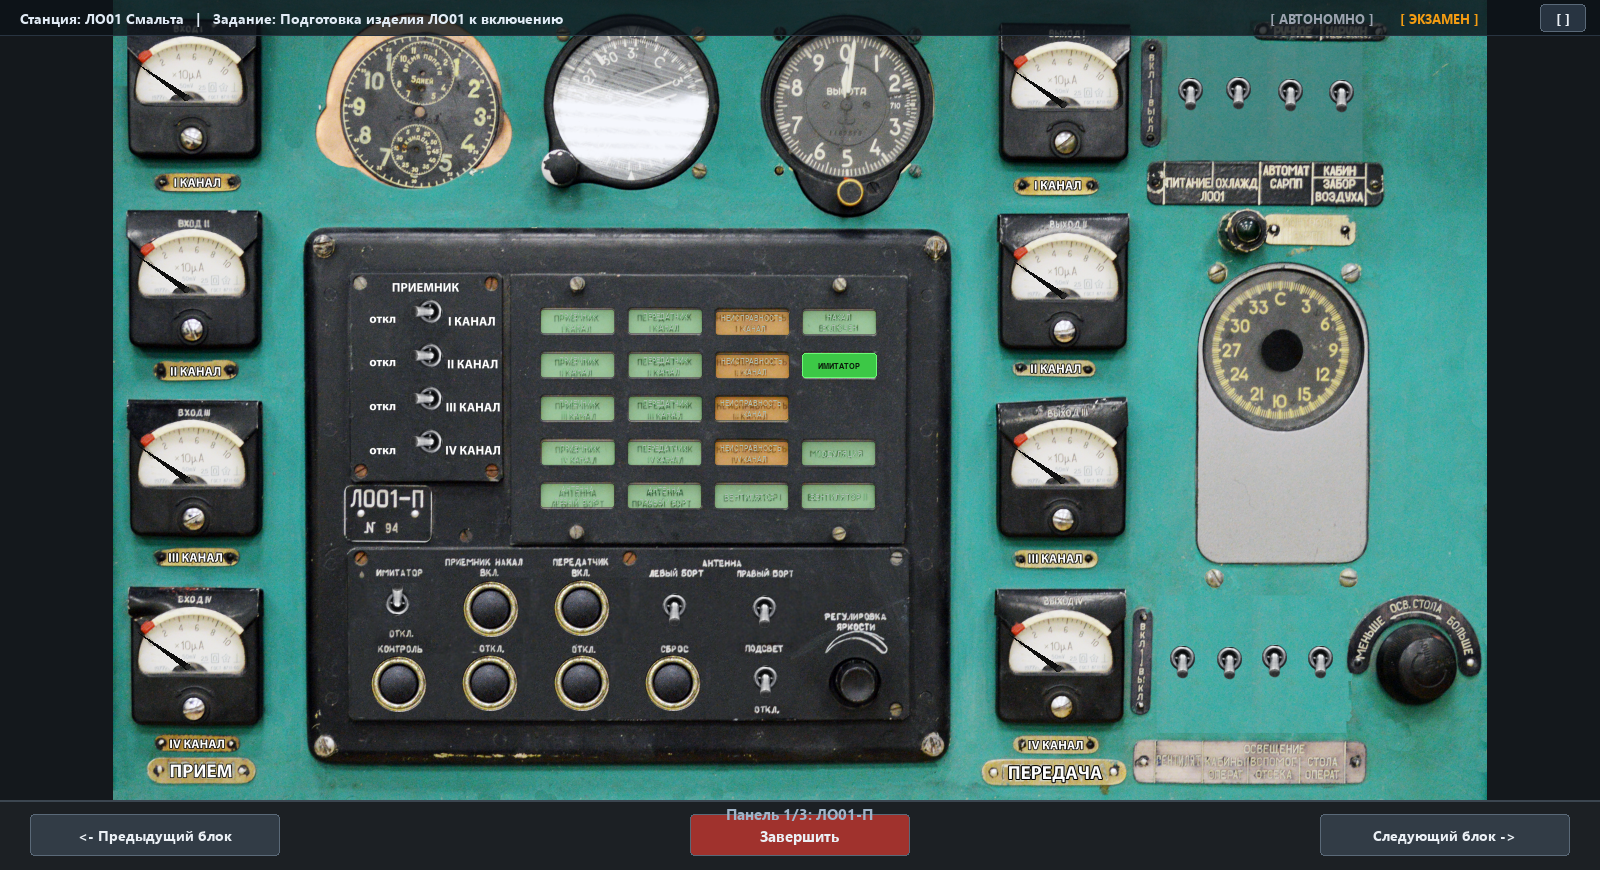
\includegraphics[width=0.95\textwidth]{04_smalta_rack.png}
    \caption{Основная рабочая панель симулятора стойки изделия Л001 («Смальта»)}
    \label{fig:smalta_rack}
\end{figure}

\section{Режимы функционирования симулятора}
Симулятор поддерживает три базовых режима работы:
\begin{enumerate}
    \item \textbf{Режим «Обучение»}: обучаемый имеет свободный доступ к пошаговым графическим подсказкам, детальному описанию каждого действия и контекстной помощи. Ошибки не приводят к штрафным баллам, позволяя оператору закрепить последовательность операций.
    \item \textbf{Режим «Экзамен» (Автономный)}: проводится без подключения к локальной вычислительной сети. Подсказки полностью заблокированы, фиксируется хронометраж и рассчитывается итоговый балл.
    \item \textbf{Режим «Сетевой Экзамен» (Архитектура «Клиент-Преподаватель»)}: ключевой режим контроля знаний. Рабочие станции курсантов подключаются по локальной сети к рабочему месту преподавателя, синхронно управляются пультом экзаменатора и передают полную телеметрию действий и скриншоты в реальном времени.
\end{enumerate}

% =========================================================================
% ГЛАВА 2: СЕТЕВАЯ АРХИТЕКТУРА И АВТОПОИСК
% =========================================================================
\chapter{Сетевая архитектура «Клиент-Преподаватель»}

\section{Топология распределённого экзаменационного класса}
Сетевой мониторинг построен по клиент-серверной топологии типа «Звезда» (рисунок~\ref{fig:net_arch}). 

\begin{figure}[H]
    \centering
    \begin{tcolorbox}[colback=white,colframe=primaryblue!60!black,arc=2mm,center,width=0.92\textwidth]
        \centering
        \textbf{АРМ ПРЕПОДАВАТЕЛЯ (\texttt{TeacherServer.exe})}\\[1mm]
        \small HTTP REST API (Порт 8000) $\bullet$ Server-Sent Events (SSE) $\bullet$ UDP Discovery Responder (Порт 50505)\\[2mm]
        $\updownarrow$ \footnotesize Локальная сеть (Wi-Fi / Ethernet / Мобильный хот-спот) $\updownarrow$\\[2mm]
        \parbox{0.28\textwidth}{\centering \textbf{АРМ Курсанта 1}\\ \scriptsize \texttt{SmaltaSim.exe}\\ Скриншоты $\bullet$ BBox}\hfill
        \parbox{0.28\textwidth}{\centering \textbf{АРМ Курсанта 2}\\ \scriptsize \texttt{SmaltaSim.exe}\\ Античит $\bullet$ Win32}\hfill
        \parbox{0.28\textwidth}{\centering \textbf{АРМ Курсанта $N$}\\ \scriptsize \texttt{SmaltaSim.exe}\\ Дедупликация}
    \end{tcolorbox}
    \caption{Схема информационного обмена в экзаменационном классе}
    \label{fig:net_arch}
\end{figure}

\begin{itemize}
    \item \textbf{Сервер экзаменатора (\texttt{TeacherServer.exe})}: функционирует без внешних тяжёлых веб-серверов (Apache/Nginx) на базе встроенного многопоточного движка. Обеспечивает отображение интерактивного веб-пульта преподавателя на HTML5/CSS3/SSE, сбор логов и архивацию снимков экрана.
    \item \textbf{Клиент курсанта (\texttt{SmaltaSim.exe})}: содержит фоновый асинхронный сетевой поток (\texttt{StudentClient}), не снижающий частоту отрисовки тренажёра (60 кадров в секунду), а также специализированный Win32-модуль отслеживания активных окон (\texttt{ScreenTracker}).
\end{itemize}

\section{Интеллектуальный 4-уровневый алгоритм автопоиска IP}
В условиях учебных классов нередко возникают сетевые проблемы: изоляция клиентов в Wi-Fi сетях (AP Isolation), блокировка широковещательного трафика роутером, динамическая смена адресов DHCP или развёртывание на базе мобильной точки доступа Windows.

Для гарантированного 100\% автоматического соединения симулятора с сервером преподавателя реализован \textbf{четырёхуровневый отказоустойчивый алгоритм автопоиска}:

\begin{enumerate}
    \item \textbf{Уровень 1: Мгновенное кэширование и Localhost ($\sim$10 мс)}.\\
    Симулятор мгновенно опрашивает последний подтверждённый адрес из локального файла \texttt{student\_profile.json}, а также адрес \texttt{127.0.0.1}. Если конфигурация класса не менялась, вход происходит без малейших задержек.
    \item \textbf{Уровень 2: Параллельный UDP Broadcast с защитой от WSAECONNRESET}.\\
    На сервере преподавателя включён низкоуровневый флаг \texttt{socket.SIO\_UDP\_CONNRESET}, предотвращающий «засыпание» слушателя при сбоях клиентов в Windows. Клиент параллельно через неблокирующий системный вызов \texttt{select.select()} опрашивает все физические адаптеры и адреса шлюзов.
    \item \textbf{Уровень 3: Анализ системного ARP-кэша Windows ($\sim$50 мс)}.\\
    Если роутер полностью блокирует широковещательный UDP-трафик, симулятор извлекает таблицу активных устройств через Win32 ARP-стек (\texttt{arp -a}), фильтрует узлы своей подсети (/24) и точечно опрашивает их.
    \item \textbf{Уровень 4: Высокоскоростное сканирование подсети /24 ($\sim$1.13 с)}.\\
    В случае абсолютной блокировки бродкаста запускается пул из 80 рабочих потоков, опрашивающих всю подсеть из 254 адресов. За 1 секунду сервер обнаруживается, верифицируется через эндпоинт \texttt{/api/ping} и автоматически сохраняется в профиль курсанта.
\end{enumerate}

\begin{tipBox}
    Симулятор официально поддерживает проведение занятий в полевых условиях с раздачей сети прямо с ноутбука преподавателя через встроенную функцию Windows «Мобильный хот-спот» (подсеть \texttt{192.168.137.*}). Наличие внешнего роутера или доступа к Интернету \textbf{не требуется}.
\end{tipBox}

% =========================================================================
% ГЛАВА 3: РАЗВЁРТЫВАНИЕ И ПОДГОТОВКА
% =========================================================================
\chapter{Порядок развёртывания и подготовка к занятию}

\section{Системные требования}
Для надёжной работы программного комплекса на рабочих станциях рекомендуется следующая аппаратная и программная конфигурация:
\begin{table}[H]
    \centering
    \begin{tabularx}{\textwidth}{lX}
        \toprule
        \textbf{Параметр} & \textbf{Рекомендуемые требования} \\
        \midrule
        Операционная система & Microsoft Windows 10 / 11 (64-бит) \\
        Процессор & Двухъядерный CPU с частотой от 2.0 ГГц \\
        Оперативная память & Не менее 2 ГБ RAM \\
        Видеоадаптер & С поддержкой аппаратного ускорения 2D/3D (DirectX 9+) \\
        Разрешение экрана & Не менее $1280 \times 720$ (оптимально: $1920 \times 1080$ Full HD) \\
        Сетевой интерфейс & Ethernet 100/1000 Мбит/с или Wi-Fi 802.11n/ac \\
        \bottomrule
    \end{tabularx}
    \caption{Системные требования комплекса SmaltaSim}
\end{table}

\section{Порядок запуска сервера преподавателя}
\begin{enumerate}
    \item На компьютере руководителя занятия запустите исполняемый файл \textbf{\texttt{TeacherServer.exe}}.
    \item Приложение автоматически откроет веб-пульт в браузере по умолчанию по адресу:
    \begin{center}
        \texttt{http://localhost:8000}
    \end{center}
    \item В шапке веб-интерфейса отобразится текущий локальный IP-адрес компьютера преподавателя в учебной сети (например, \texttt{IP: 192.168.1.45:8000}).
\end{enumerate}

\section{Порядок запуска симулятора на местах курсантов}
\begin{enumerate}
    \item На рабочих местах курсантов запустите исполняемый файл \textbf{\texttt{SmaltaSim.exe}}.
    \item В главном меню (рисунок~\ref{fig:main_menu}) выберите пункт \textbf{«Экзамен»}.
    \item В открывшемся окне авторизации (рисунок~\ref{fig:auth_dialog}) курсант вводит:
    \begin{itemize}
        \item Своё полное \textbf{ФИО};
        \item Номер учебного \textbf{взвода / группы};
        \item Название рабочего места (АРМ подставляется автоматически);
        \item IP-адрес сервера (определяется автоматически; при необходимости может быть скорректирован вручную).
    \end{itemize}
    \item После подтверждения данных курсант выбирает учебный билет.
    \item Симулятор переходит в защищённый режим ожидания (рисунок~\ref{fig:waiting_dialog}), блокируя доступ к органам управления до момента подачи преподавателем команды «Старт».
\end{enumerate}

\begin{figure}[H]
    \centering
    \begin{minipage}{0.48\textwidth}
        \centering
        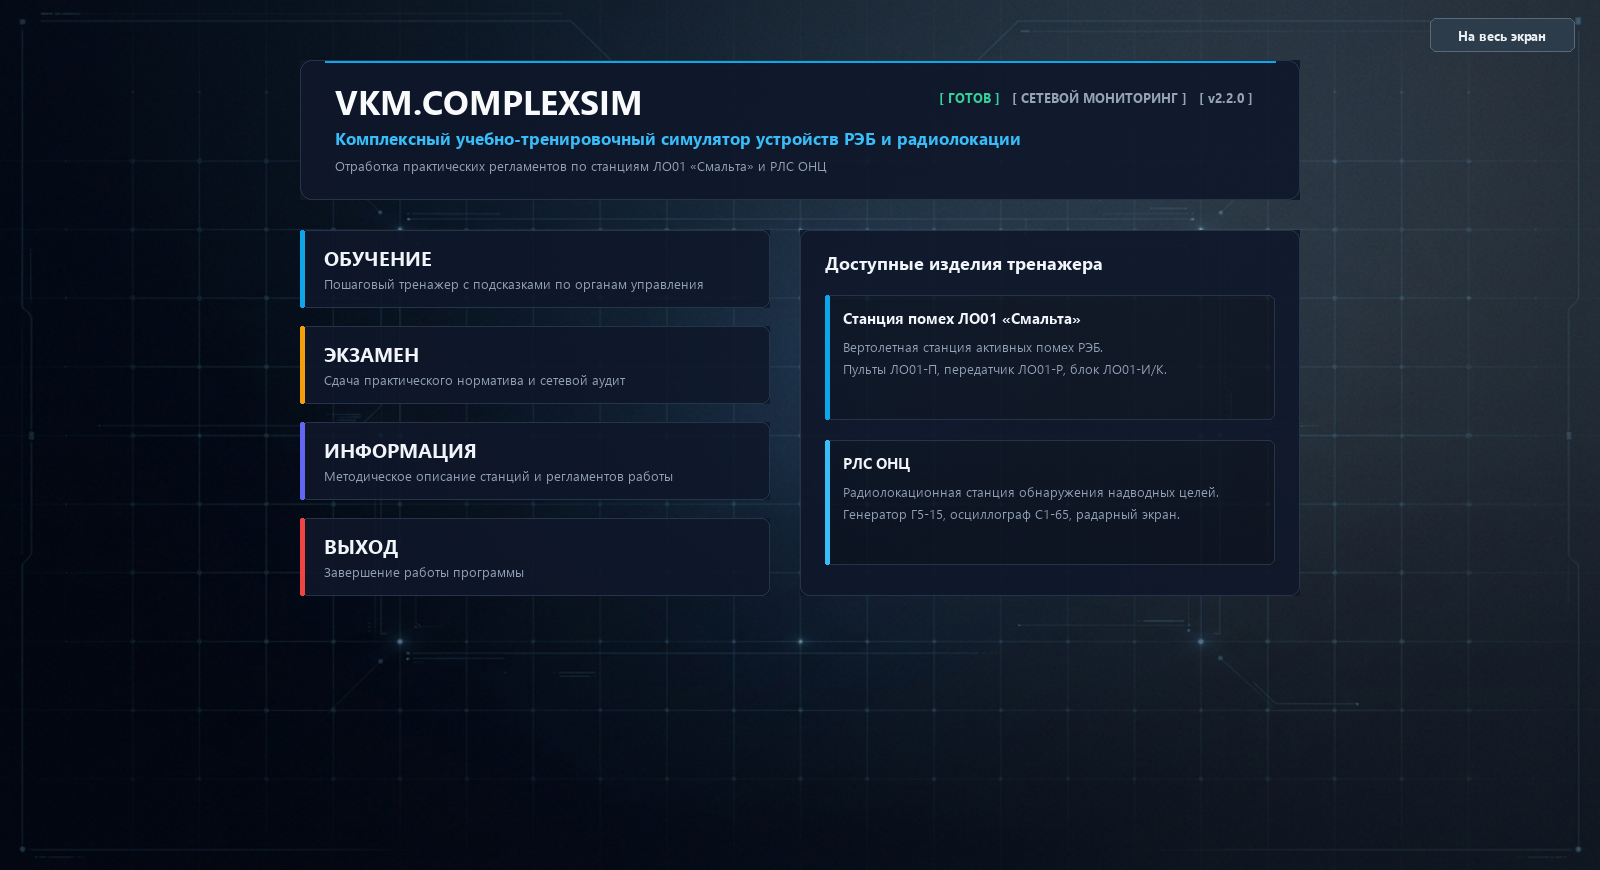
\includegraphics[width=\textwidth]{01_main_menu.png}
        \caption{Главное меню симулятора}
        \label{fig:main_menu}
    \end{minipage}\hfill
    \begin{minipage}{0.48\textwidth}
        \centering
        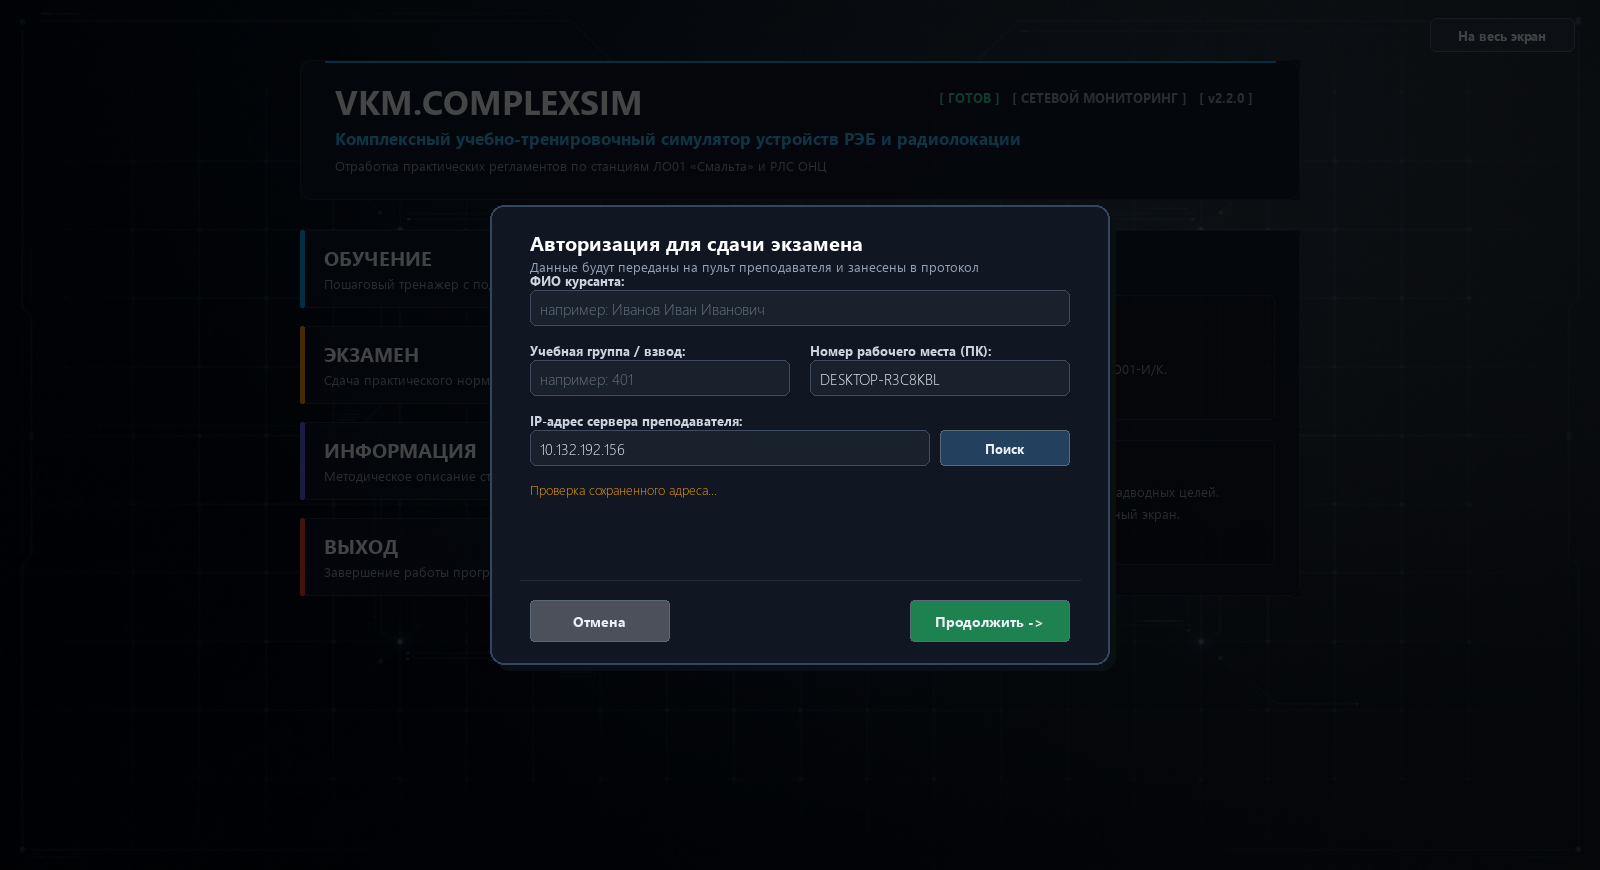
\includegraphics[width=\textwidth]{02_auth_dialog.png}
        \caption{Окно авторизации курсанта}
        \label{fig:auth_dialog}
    \end{minipage}
\end{figure}

\begin{figure}[H]
    \centering
    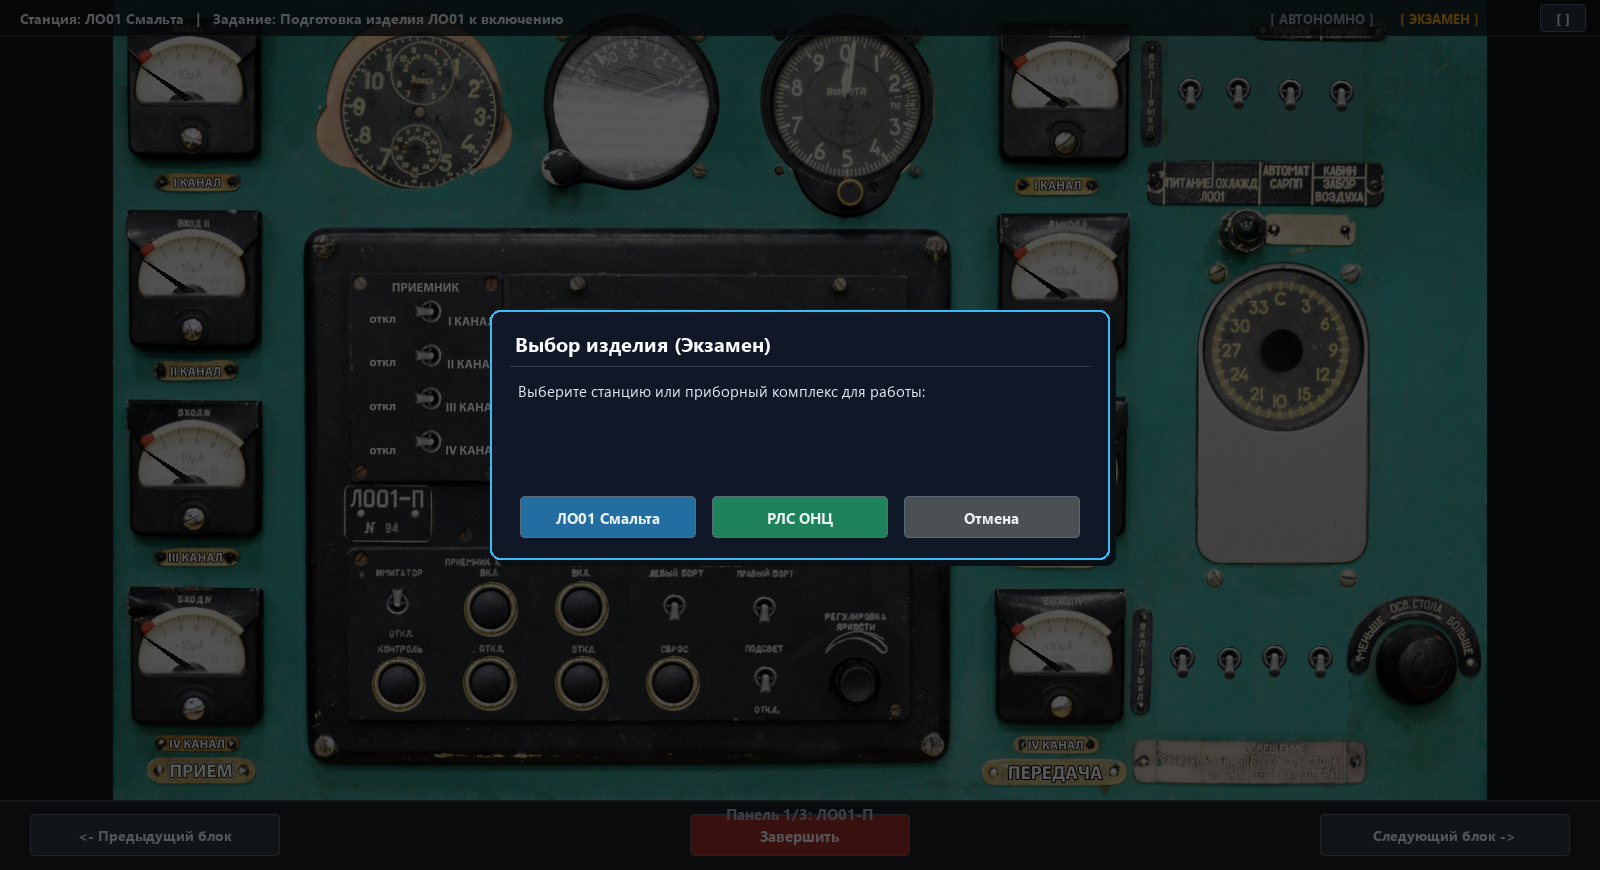
\includegraphics[width=0.7\textwidth]{03_waiting_dialog.png}
    \caption{Окно блокировки в ожидании допуска преподавателя}
    \label{fig:waiting_dialog}
\end{figure}

% =========================================================================
% ГЛАВА 4: РАБОТА В СИМУЛЯТОРЕ КУРСАНТА
% =========================================================================
\chapter{Порядок работы курсанта и правила выполнения билета}

\section{Навигация по блокам и манипуляция элементами}
Комплекс «Смальта» состоит из нескольких пространственных секций. Навигация осуществляется:
\begin{itemize}
    \item Кнопками нижней навигационной панели \textbf{«<- Предыдущий блок»} и \textbf{«Следующий блок ->»};
    \item Клавишами клавиатуры \texttt{Left} / \texttt{Right} или колесом мыши.
\end{itemize}

Все органы управления (тумблеры, кнопки, галетные переключатели) обладают визуальным эффектом упругости: при нажатии курсором мыши элемент анимированно переключается и воспроизводит соответствующее механическое состояние.

\section{Механизм защиты от ложных ошибок (Дедупликация тумблеров)}
\begin{infoNote}
    В реальной работе со сложной военной техникой оператор при переводе трёхпозиционного или многопозиционного переключателя (например, из положения «ОТКЛ» в положение «II КАНАЛ») неизбежно кратковременно проходит промежуточные положения («I КАНАЛ»).
\end{infoNote}

В симуляторе версии 2.2.0 внедрён специальный алгоритм \textbf{отложенной фиксации ошибок}:
\begin{itemize}
    \item Промежуточные переключения одного и того же органа управления \textbf{не штрафуются};
    \item Фиксация правильности или ошибочности действия происходит \textbf{только в момент перехода оператора к следующему этапу алгоритма};
    \item Если курсант ошибочно щёлкнул тумблером, но до нажатия других органов управления вернул его в требуемое исходное положение, штрафная ошибка \textbf{не засчитывается}.
\end{itemize}

\section{Завершение экзамена}
После выполнения последнего шага алгоритма или при нажатии кнопки «Завершить» симулятор производит автоматический расчёт и выводит модальное окно с результатами (рисунок~\ref{fig:exam_results}).

\begin{figure}[H]
    \centering
    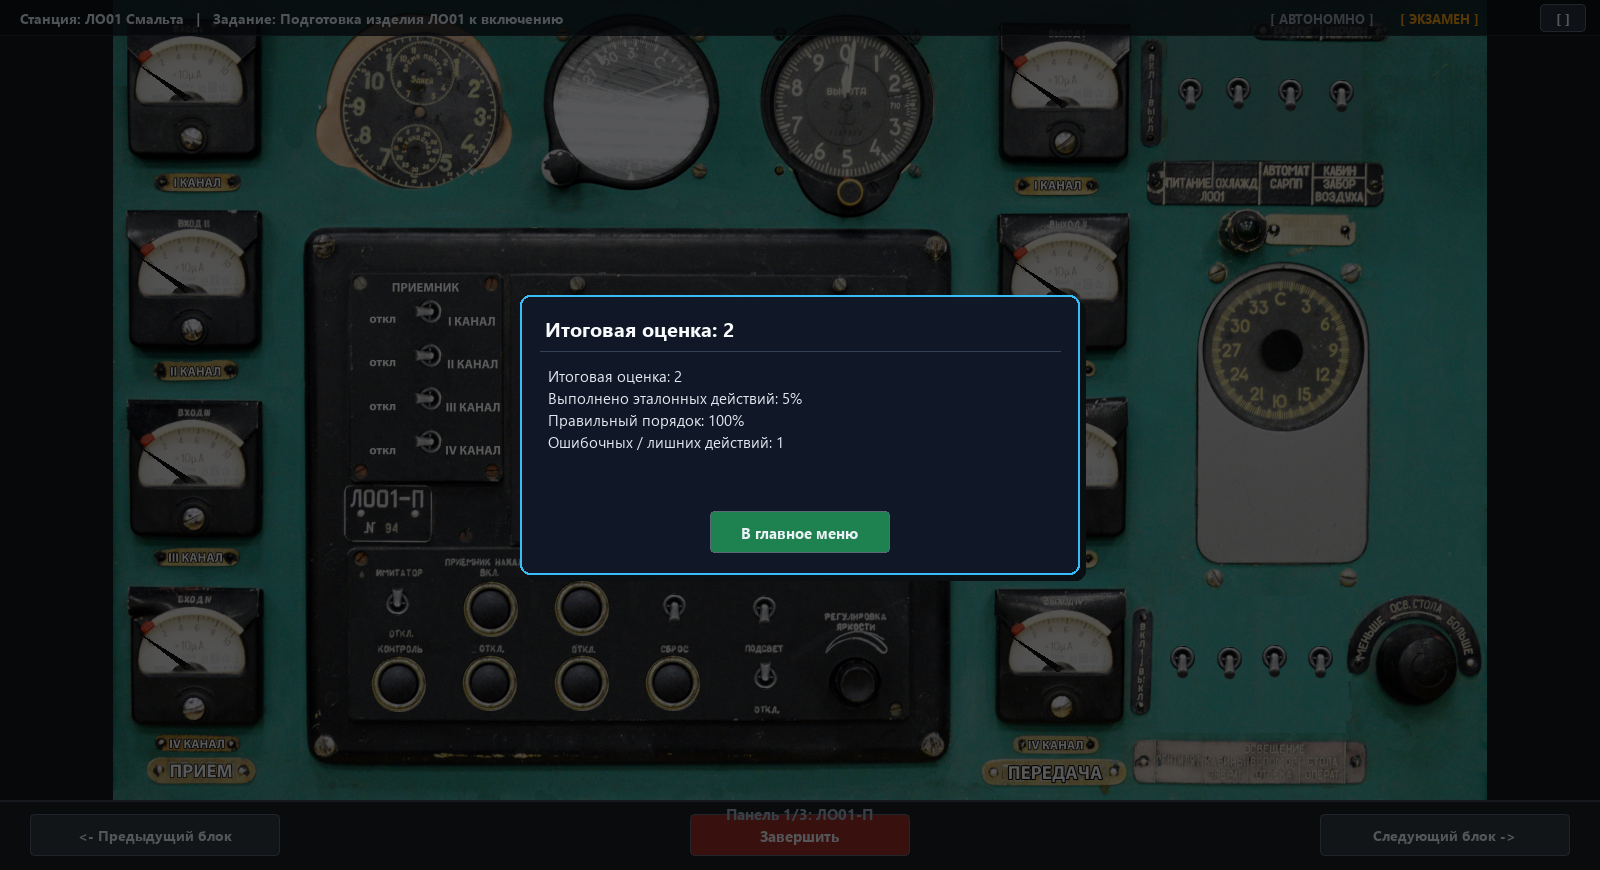
\includegraphics[width=0.75\textwidth]{07_exam_results.png}
    \caption{Итоговое окно результатов с однозначной оценкой}
    \label{fig:exam_results}
\end{figure}

% =========================================================================
% ГЛАВА 5: АНТИЧИТ И АННОТИРОВАНИЕ
% =========================================================================
\chapter{Система фиксации действий, скриншотов и античит-контроля}

\section{Аннотированные снимки с ограничивающими рамками (BBox)}
При каждом действии курсанта (как успешном, так и ошибочном) симулятор генерирует высококачественный графический срез экрана с наложением интеллектуальной векторной разметки:
\begin{itemize}
    \item \textbf{Правильное действие}: требуемый орган управления обводится \textbf{зелёным контуром} с подтверждающей индикацией (рисунок~\ref{fig:correct_action}).
    \item \textbf{Ошибочное действие}: неверно нажатый элемент подсвечивается \textbf{ярким красным контуром}, целевой элемент выделяется \textbf{зелёным контуром}, а в верхней части кадра формируется контрастный информационный баннер с точным указанием шага алгоритма, допущенной ошибки и требуемого действия (рисунок~\ref{fig:mistake_action}).
\end{itemize}

\begin{figure}[H]
    \centering
    \begin{minipage}{0.48\textwidth}
        \centering
        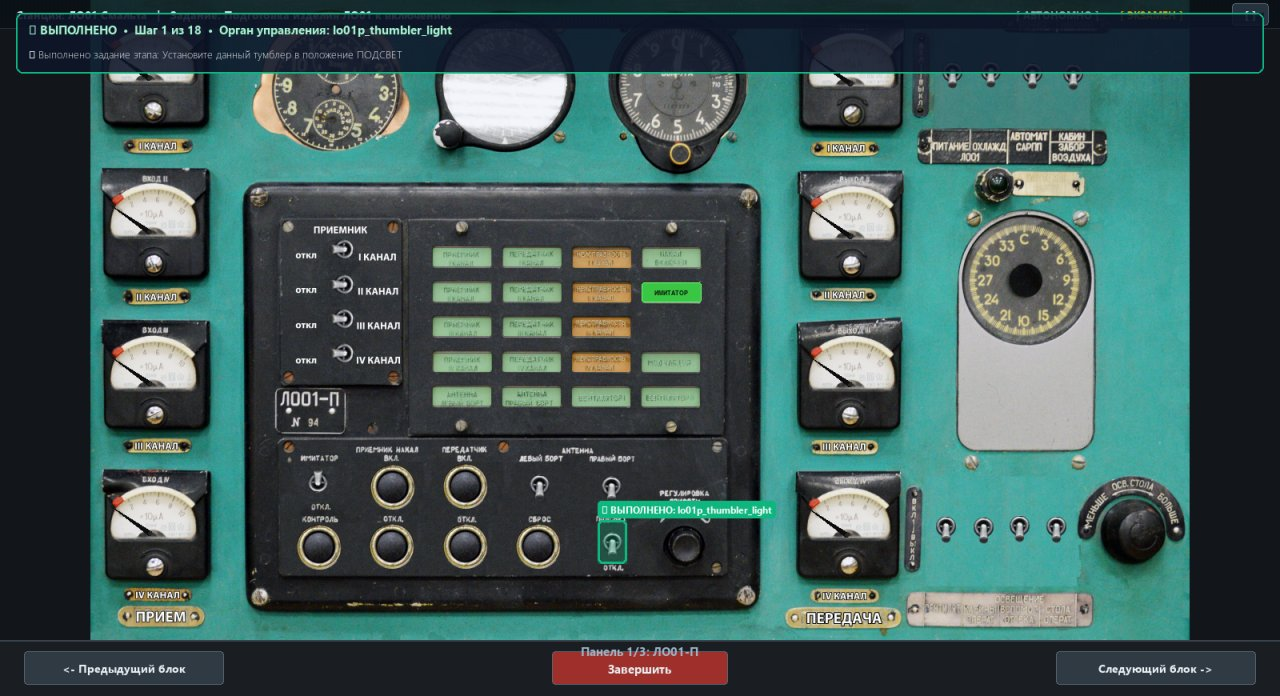
\includegraphics[width=\textwidth]{05_action_correct.png}
        \caption{Фиксация правильного действия (Зелёный BBox)}
        \label{fig:correct_action}
    \end{minipage}\hfill
    \begin{minipage}{0.48\textwidth}
        \centering
        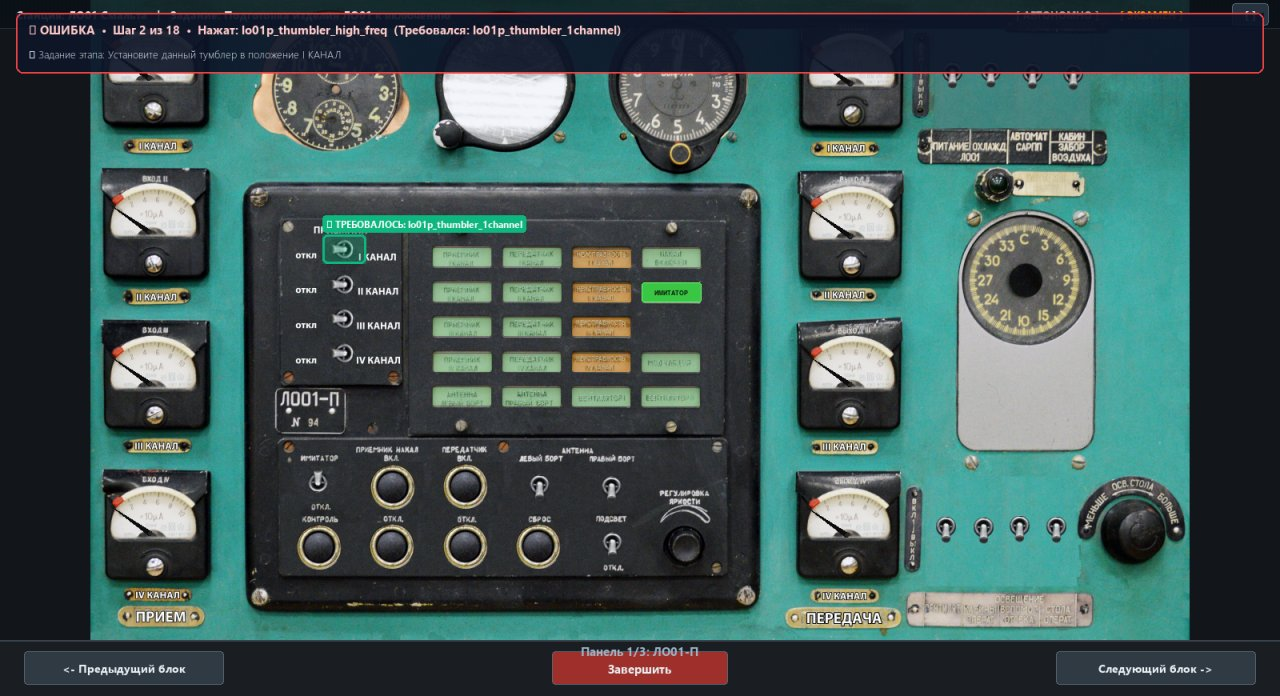
\includegraphics[width=\textwidth]{06_action_mistake.png}
        \caption{Фиксация ошибки с указанием шага и целевого элемента}
        \label{fig:mistake_action}
    \end{minipage}
\end{figure}

\section{Система контроля экрана и античит}
Для предотвращения использования обучаемыми электронных шпаргалок, конспектов в формате PDF, браузеров и мессенджеров во время сдачи экзамена, в симулятор интегрирован специализированный модуль контроля рабочего стола:
\begin{itemize}
    \item \textbf{Перехват фокуса Windows}: симулятор мгновенно фиксирует сворачивание окна или переход курсора на стороннее приложение через вызовы Win32 API (\texttt{GetForegroundWindow}, \texttt{GetWindowTextW}).
    \item \textbf{Идентификация программы}: в журнал преподавателя отправляется \textbf{точное название стороннего окна} (например: \textit{«Google Chrome --- Конспект\_Смальта\_Лекция4.pdf»}).
    \item \textbf{Скриншот всего экрана}: фоновый агент выполняет захват реального рабочего стола Windows (через GDI BitBlt), благодаря чему преподаватель видит, что именно открыл курсант поверх симулятора.
    \item \textbf{Хронометраж отвлечений}: карточка курсанта на пульте начинает пульсировать тревожным цветом, а система накапливает точное число секунд нахождения вне тренажёра.
\end{itemize}

\begin{warnBox}
    При попытке курсанта свернуть симулятор карточка рабочего места на пульте преподавателя мгновенно окрашивается в оранжево-красный цвет с указанием названия открытого документа.
\end{warnBox}

% =========================================================================
% ГЛАВА 6: РАБОТА ПРЕПОДАВАТЕЛЯ
% =========================================================================
\chapter{Методика проведения экзамена (Пульт преподавателя)}

\section{Обзор веб-интерфейса пульта}
Веб-пульт преподавателя (рисунок~\ref{fig:teacher_dash}) разработан с учётом требований эргономики современных центров управления. Верхняя информационная панель отображает сводную статистику по классу:
\begin{itemize}
    \item Общее количество подключённых курсантов;
    \item Количество курсантов, сдающих в данный момент;
    \item Суммарное количество зафиксированных ошибок;
    \item Количество успешно завершивших экзамен.
\end{itemize}

\begin{figure}[H]
    \centering
    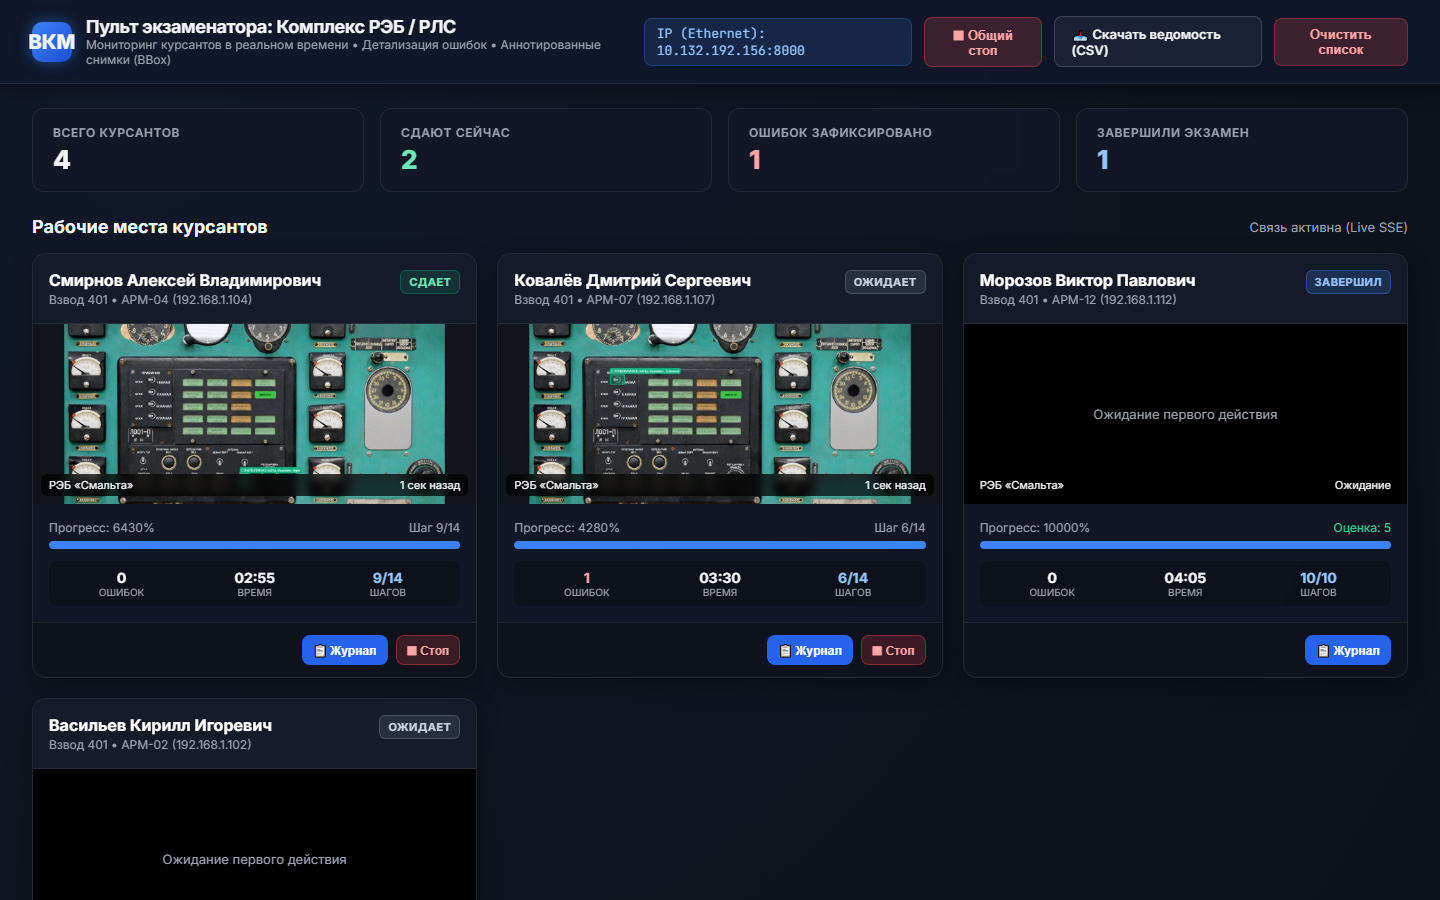
\includegraphics[width=0.98\textwidth]{08_teacher_dashboard.png}
    \caption{Главный экран веб-пульта экзаменатора (карточки рабочих мест)}
    \label{fig:teacher_dash}
\end{figure}

\section{Управление ходом экзамена}
Преподаватель имеет в своём распоряжении два механизма запуска:
\begin{enumerate}
    \item \textbf{Кнопка «Общий старт»}: одновременно отправляет сетевой сигнал допуска на все подключённые рабочие места, находящиеся в режиме ожидания. На всех компьютерах курсантов мгновенно закрывается окно блокировки и включается таймер.
    \item \textbf{Кнопка «Начать» на индивидуальной карточке}: позволяет запустить экзамен конкретному курсанту (например, при опоздании или индивидуальной пересдаче).
    \item \textbf{Кнопка «Стоп»}: принудительно останавливает экзамен конкретного курсанта. На компьютере обучаемого симулятор прекращает работу и выводит сообщение о досрочном завершении преподавателем.
\end{enumerate}

\section{Инспекция журнала действий курсанта}
При нажатии на кнопку \textbf{«Журнал»} на карточке обучаемого открывается детальное модальное окно (рисунок~\ref{fig:student_modal}). В окне представлены:
\begin{itemize}
    \item Таб \textbf{«Общий лог»}: поминутная хронология всех манипуляций тумблерами и кнопками;
    \item Таб \textbf{«Лог ошибок»}: отфильтрованный список только некорректных действий с пояснениями;
    \item События безопасности \textbf{«[ВНИМАНИЕ]»}: факты переключения на сторонние окна с временной меткой.
\end{itemize}

\begin{figure}[H]
    \centering
    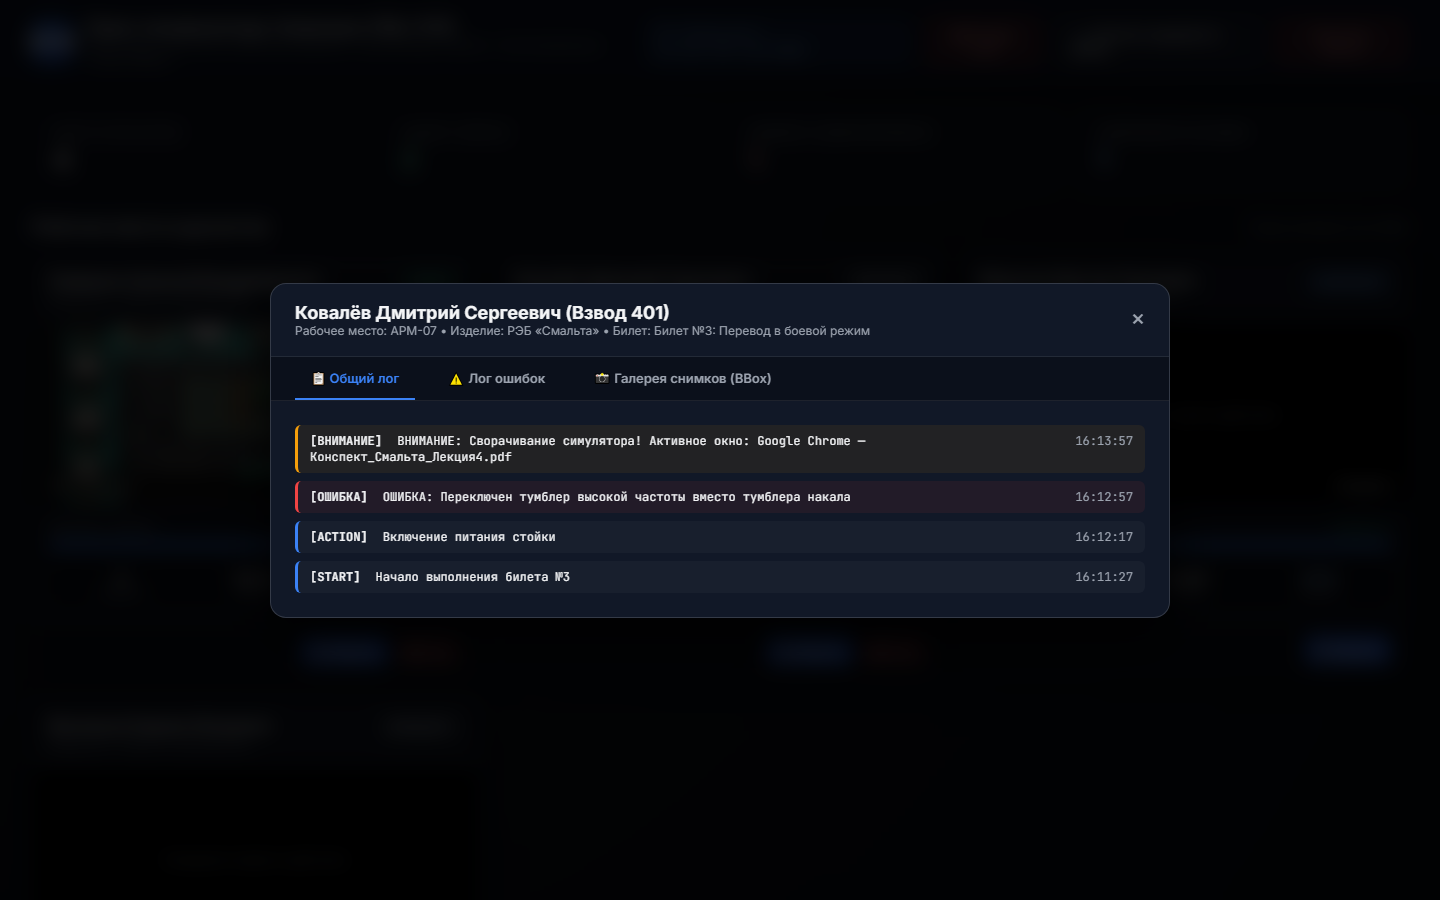
\includegraphics[width=0.85\textwidth]{09_teacher_student_modal.png}
    \caption{Модальное окно курсанта: журнал действий и событий античита}
    \label{fig:student_modal}
\end{figure}

\section{Галерея снимков экрана и полноэкранный зум}
Перейдя на вкладку \textbf{«Галерея снимков (BBox)»} (рисунок~\ref{fig:gallery_modal}), преподаватель может просмотреть визуальную ленту скриншотов рабочего места курсанта. 
Клик по любому снимку открывает его в полноэкранном масштабе, позволяя до мельчайших деталей изучить положение тумблеров и показания приборов в момент совершения ошибки.

\begin{figure}[H]
    \centering
    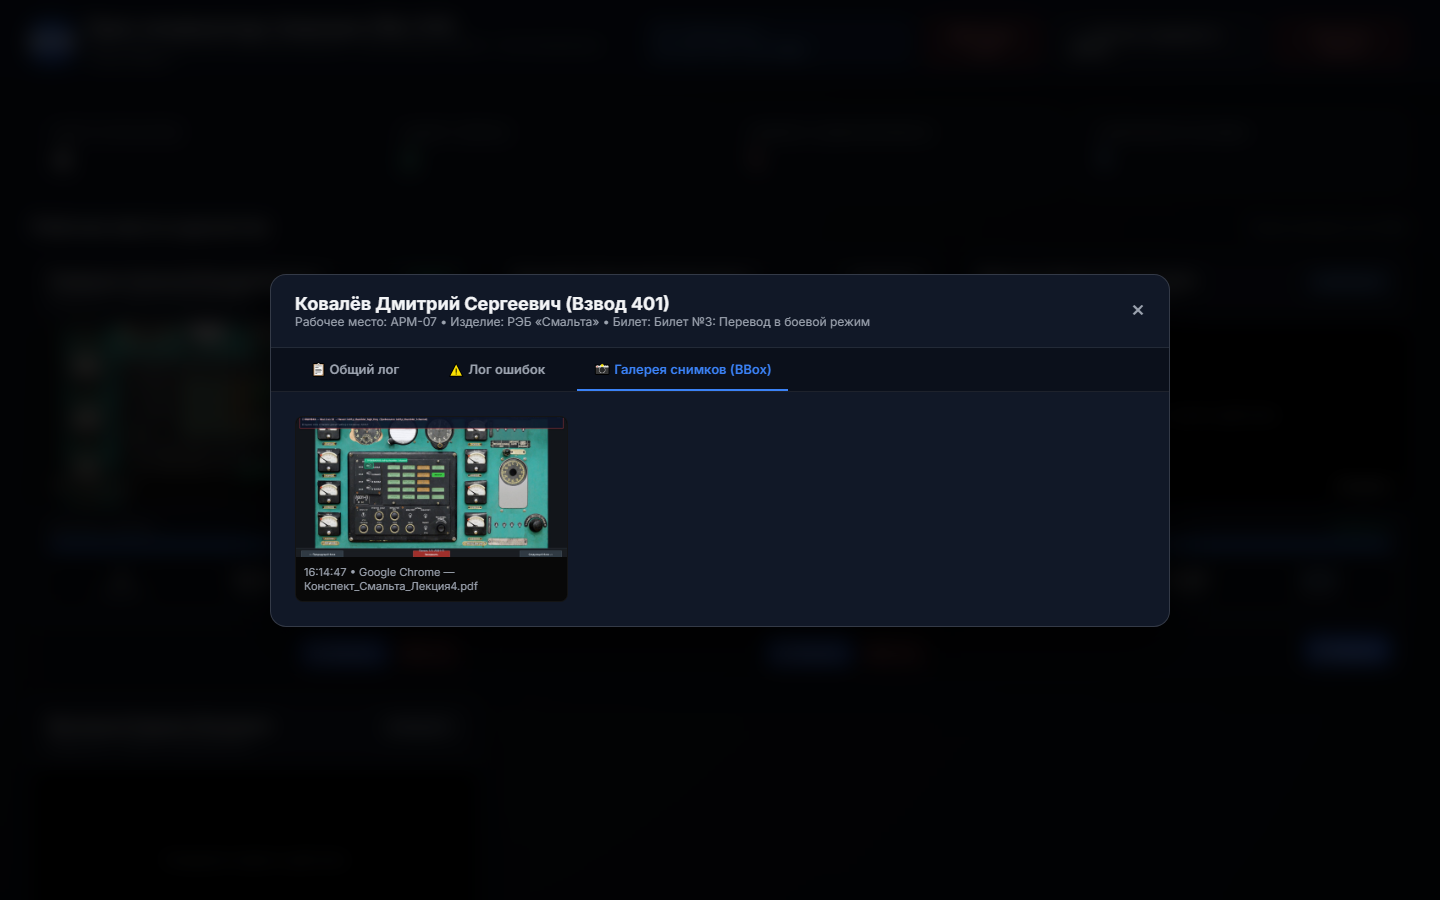
\includegraphics[width=0.85\textwidth]{10_teacher_gallery_modal.png}
    \caption{Галерея снимков экрана с фиксацией рабочих окон}
    \label{fig:gallery_modal}
\end{figure}

\section{Экспорт экзаменационной ведомости (CSV)}
По окончании экзаменационного занятия преподаватель нажимает кнопку \textbf{«Скачать ведомость (CSV)»}. 
Формируется структурированный отчёт с кодировкой UTF-8 BOM (полностью совместимый с Microsoft Excel, LibreOffice Calc и 1С):

\begin{table}[H]
    \centering
    \small
    \begin{tabularx}{\textwidth}{lcccc}
        \toprule
        \textbf{ФИО курсанта} & \textbf{Взвод / ПК} & \textbf{Оценка} & \textbf{Ошибок} & \textbf{Время (с)} \\
        \midrule
        Смирнов Алексей Владимирович & 401 / АРМ-04 & \textbf{5} & 0 & 175 \\
        Ковалёв Дмитрий Сергеевич & 401 / АРМ-07 & \textbf{4} & 1 & 210 \\
        Морозов Виктор Павлович & 401 / АРМ-12 & \textbf{5} & 0 & 245 \\
        Васильев Кирилл Игоревич & 401 / АРМ-02 & \textbf{3} & 4 & 310 \\
        \bottomrule
    \end{tabularx}
    \caption{Пример структуры сформированной экзаменационной ведомости}
\end{table}

% =========================================================================
% ГЛАВА 7: КРИТЕРИИ ОЦЕНИВАНИЯ
% =========================================================================
\chapter{Критерии и шкала оценивания знаний}

\section{Правила выставления итоговой оценки}
В программном комплексе версии 2.2.0 утверждена строгая объективная 4-уровневая шкала оценивания, исключающая субъективный фактор. Итоговая оценка формируется автоматически на основании полноты выполнения эталона и количества штрафных ошибок:

\begin{table}[H]
    \centering
    \begin{tabularx}{\textwidth}{ccX}
        \toprule
        \textbf{Оценка} & \textbf{Кол-во ошибок} & \textbf{Условия выставления} \\
        \midrule
        \textbf{\Huge 5} & \textbf{0} & Алгоритм билета выполнен в полном объёме (100\%) без единой ошибки. Все коммутации выполнены строго по инструкции. \\
        \addlinespace
        \textbf{\Huge 4} & \textbf{1 -- 3} & Алгоритм билета выполнен на 100\%, при этом допущено от одной до трёх некритических ошибок, своевременно исправленных обучаемым. \\
        \addlinespace
        \textbf{\Huge 3} & \textbf{4 и более} & Экзамен выполнен на 100\% независимо от общего числа допущенных ошибок (при условии доведения изделия до работоспособного состояния). \\
        \addlinespace
        \textbf{\Huge 2} & --- & Алгоритм не завершён обучаемым, либо экзамен был принудительно остановлен руководителем за нарушение дисциплины. \\
        \bottomrule
    \end{tabularx}
    \caption{Шкала критериев оценивания обучаемых в симуляторе SmaltaSim}
\end{table}

\begin{infoNote}
    \begin{itemize}
        \item Оценка «1» (единица) в системе \textbf{не используется}.
        \item На экране обучаемого и в протоколе преподавателя оценка выводится \textbf{строго в виде однозначной цифры} (без текстовых формулировок вроде «Хорошо» или «Неуд»).
    \end{itemize}
\end{infoNote}

% =========================================================================
% ГЛАВА 8: УСТРАНЕНИЕ НЕПОЛАДОК
% =========================================================================
\chapter{Диагностика и устранение неисправностей (FAQ)}

\section{Типовые сетевые неисправности и их решение}

\subsection{Симулятор курсанта не находит сервер автоматически}
\begin{enumerate}
    \item Проверьте, запущен ли \texttt{TeacherServer.exe} на компьютере преподавателя.
    \item Убедитесь, что компьютеры курсанта и преподавателя подключены к одной локальной сети (одному Wi-Fi роутеру или коммутатору).
    \item Если на компьютерах включён Брандмауэр Windows (Windows Defender Firewall), проверьте, разрешён ли входящий и исходящий трафик:
    \begin{itemize}
        \item Протокол \textbf{TCP}: порт \textbf{8000} (веб-интерфейс и API);
        \item Протокол \textbf{UDP}: порт \textbf{50505} (широковещательный поиск).
    \end{itemize}
    \item При необходимости в окне авторизации курсанта введите IP-адрес сервера вручную (он указан в шапке браузера преподавателя).
\end{enumerate}

\subsection{Курсант случайно закрыл приложение во время экзамена}
При повторном запуске \texttt{SmaltaSim.exe} курсант вводит своё прежнее ФИО. Симулятор восстановит соединение с сервером преподавателя, а в журнале будет зафиксировано событие повторного входа без потери ранее зарегистрированных скриншотов.

\section{Горячие клавиши симулятора}
\begin{itemize}
    \item \texttt{F11} --- переключение между полноэкранным и оконным режимами;
    \item \texttt{Esc} --- закрытие текущего диалогового окна или возврат в главное меню;
    \item \texttt{Left} / \texttt{Right} --- быстрая навигация между блоками аппаратуры.
\end{itemize}

% =========================================================================
% ЗАКЛЮЧЕНИЕ
% =========================================================================
\chapter*{Заключение}
\addcontentsline{toc}{chapter}{Заключение}

Внедрение программного комплекса имитационного моделирования \textbf{SmaltaSim v2.2.0} обеспечивает переход учебного процесса на качественно новый технологический уровень. 

Связка симулятора рабочего места с веб-пультом преподавателя, автоматизированный античит-контроль, детализация ошибок с векторными рамками (BBox) и объективная шкала оценивания позволяют проводить объективные срезы знаний с минимальными трудозатратами со стороны преподавательского состава.

\end{document}
